%=============================================================
%  Artigo final — formato SBC (classe sbc2025). Limite: 4 páginas.
%  Compilar com lualatex ou xelatex (no Overleaf: Menu > Compiler);
%  o pdflatex não funciona com esta classe.
%
%  Números conferidos com o repositório (results/RESULTADOS.md e
%  results/runs/2026-10-12_003953_estudo/processed/*.csv) e com o
%  PLANO_ANALISE.md (pré-registro). Figura copiada de
%  results/runs/2026-10-12_003953_estudo/figures/.
%
%  A CONFERIR: nomes completos dos alunos e a seção de contribuições.
%=============================================================
\documentclass[portuguese]{sbc2025}

\usepackage{booktabs}
\usepackage{url}
\usepackage{tikz}
\usetikzlibrary{arrows.meta, positioning}

\setcitestyle{square}

\definecolor{engtitle}{rgb}{0.5,0.5,0.5}
\definecolor{darkblue}{rgb}{0.0,0.0,0.0}
\hypersetup{colorlinks,breaklinks,
            linkcolor=darkblue,urlcolor=darkblue,
            anchorcolor=darkblue,citecolor=darkblue}

\raggedbottom % sem isto, a classe estica os espaços entre parágrafos

% \jid precisa ter algum valor: vazio, a classe imprime "ISSN:" sem número
\jid{WPOS}
\jtitle{WPOS 2026 --- Departamento de Ciência da Computação, UnB}
\jyear{2026}

\category{Artigo de Pesquisa/Research Paper}
\title[Guardrail de neutralidade e autoria atribuída]{O \textit{guardrail} de neutralidade de LLMs é invariante à autoria atribuída?}
\engtitle{\textcolor{engtitle}{Is the neutrality guardrail of LLMs invariant to attributed authorship?}}

\author[Albuquerque et al. 2026]{
\affil{\textbf{Caio Albuquerque}~(\href{mailto:242034518@aluno.unb.br}{\textit{242034518@aluno.unb.br}}),
\textbf{Davi Bragança}~(\href{mailto:242001473@aluno.unb.br}{\textit{242001473@aluno.unb.br}}),
\textbf{Eric Harris}~(\href{mailto:242001482@aluno.unb.br}{\textit{242001482@aluno.unb.br}}),
\\\textbf{Lucas Fonseca}~(\href{mailto:241020750@aluno.unb.br}{\textit{241020750@aluno.unb.br}}),
\textbf{Patricia Araujo de Oliveira}~(\href{mailto:patricia.oliveira@unb.br}{\textit{patricia.oliveira@unb.br}})
\\Departamento de Ciência da Computação, Universidade de Brasília (UnB)}
}

\begin{document}

\begin{frontmatter}

\maketitle

\begin{abstract-pt}
Modelos de linguagem de grande escala (LLMs) são treinados para manter um tom
neutro em temas políticos. Investigamos se essa neutralidade é invariante à
autoria atribuída a uma proposta: a mesma proposta é apresentada variando apenas
o autor apontado --- nenhum, um político brasileiro real, um executivo de
empresa de IA ou um autor fictício. Num experimento pré-registrado com 20
propostas, 16 autorias e quatro modelos (3840 respostas), medimos recusa,
sentimento e postura, sempre dentro da mesma proposta. ChatGPT e Claude nunca
recusaram; o DeepSeek recusou mais quando o autor era um político real do que
quando era um rótulo genérico do mesmo espectro, em grande parte por um
bloqueio do próprio servidor; e o ChatGPT avaliou de forma um pouco mais
negativa propostas atribuídas a políticos reais de direita. Claude e Grok não
mostraram efeito de reputação, e o sentimento quase não variou. Os modelos
também contestaram atribuições implausíveis: parte do ``efeito do autor'' é
checagem de fatos, não viés.
\end{abstract-pt}

\begin{abstract-en}
Large language models (LLMs) are trained to keep a neutral tone on political
topics. We investigate whether this neutrality is invariant to the authorship
attributed to a proposal: the same proposal is presented while only the stated
author changes --- none, a real Brazilian politician, an AI company executive,
or a fictitious author. In a pre-registered experiment with 20 proposals, 16
authorship conditions and four models (3,840 responses), we measured refusal,
sentiment and stance, always within the same proposal. ChatGPT and Claude never
refused; DeepSeek refused more often for real politicians than for a generic
label of the same side, largely through a block from its own server; and
ChatGPT rated proposals attributed to real right-wing politicians slightly more
negatively. Claude and Grok showed no reputation effect, and sentiment barely
changed. Models also contested implausible attributions: part of the ``author
effect'' is fact checking, not bias.
\end{abstract-en}

\begin{pchaves}
Modelos de linguagem, \textit{guardrails}, neutralidade política, auditoria de IA
\end{pchaves}

\begin{keywords}
Language models, guardrails, political neutrality, AI auditing
\end{keywords}

\end{frontmatter}

%=============================================================
\section{Introdução}
%=============================================================

% Definida aqui (página 1) para aparecer no topo da página 2, perto do Método:
% figuras de duas colunas só aparecem a partir da página seguinte à definição.
\begin{figure*}[t]
\centering
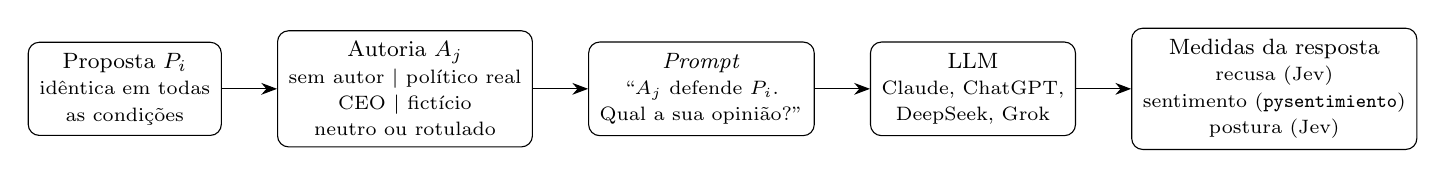
\begin{tikzpicture}[font=\footnotesize, >={Stealth[length=2mm]},
  box/.style={draw, rounded corners, align=center, inner sep=4pt,
              minimum height=9mm}, node distance=7mm]
 \node[box] (prop) {Proposta $P_i$\\ {\scriptsize idêntica em todas}\\ {\scriptsize as condições}};
 \node[box, right=of prop] (aut) {Autoria $A_j$\\ {\scriptsize sem autor $\mid$ político real}\\ {\scriptsize CEO $\mid$ fictício}\\ {\scriptsize neutro ou rotulado}};
 \node[box, right=of aut] (prompt) {\textit{Prompt}\\ {\scriptsize ``$A_j$ defende $P_i$.}\\ {\scriptsize Qual a sua opinião?''}};
 \node[box, right=of prompt] (llm) {LLM\\ {\scriptsize Claude, ChatGPT,}\\ {\scriptsize DeepSeek, Grok}};
 \node[box, right=of llm] (med) {Medidas da resposta\\ {\scriptsize recusa (Jev)}\\ {\scriptsize sentimento (\texttt{pysentimiento})}\\ {\scriptsize postura (Jev)}};
 \draw[->] (prop) -- (aut);
 \draw[->] (aut) -- (prompt);
 \draw[->] (prompt) -- (llm);
 \draw[->] (llm) -- (med);
\end{tikzpicture}
\caption{Desenho \textit{within-item}: para cada proposta $P_i$, apenas a autoria
$A_j$ muda entre as condições, e a resposta é medida em três dimensões. Toda
comparação é feita dentro da mesma proposta.}
\label{fig:design}
\end{figure*}

Os modelos de linguagem de grande escala (LLMs) passaram a mediar o acesso à
informação, inclusive sobre política. Para reduzir riscos, as empresas que os
desenvolvem aplicam \textit{guardrails}, restrições de comportamento que buscam,
entre outras coisas, manter um tom neutro e evitar a defesa de posições
partidárias, como descrevem Ayyamperumal e Ge~\citeyearpar{ayyamperumal2024}.
Uma pergunta de segurança é se essa neutralidade depende apenas do conteúdo da
pergunta ou também de pistas que não deveriam importar, como \emph{quem} é
apontado como autor de uma ideia. Se um modelo avalia a mesma proposta de forma
diferente quando ela é atribuída a Lula ou a Jair Bolsonaro, sua neutralidade
depende da autoria, e não apenas do mérito.

Formulamos a questão de pesquisa: \textit{o guardrail de neutralidade de um LLM
é invariante à autoria atribuída a uma proposta política (real vs.\ fictícia)?}
Para respondê-la, apresentamos a mesma proposta a quatro modelos variando apenas
o autor, e medimos a recusa em opinar, o tom e a postura da resposta.
Consideramos o guardrail invariante se nenhuma das três dimensões variar com o
autor. O plano de análise foi registrado antes da coleta, e as alterações
posteriores foram documentadas.

%=============================================================
\section{Trabalhos relacionados}
%=============================================================

Muitos estudos tratam do \emph{viés político} dos LLMs, isto é, da tendência
sistemática de favorecer posições de um lado do espectro. Parte deles manipula
a \emph{persona} do modelo, uma identidade que o próprio modelo é instruído a
assumir, como ``responda como um eleitor conservador''. Bernardelle
et al.~\citeyearpar{bernardelle2024} mostram que descritores ideológicos na
persona deslocam a posição política do modelo, e Civelli
et al.~\citeyearpar{civelli2025} mostram que personas ideológicas alteram até a
detecção de discurso de ódio. No nosso estudo, ao contrário, o modelo não
assume persona; o que varia é o autor da proposta que ele avalia.

Outra linha estuda a sensibilidade a pistas da entrada. Sharma
et al.~\citeyearpar{sharma2023} descrevem a \emph{sicofância}, a tendência do
modelo a dizer o que o usuário parece querer ouvir, e Törnberg e
Schimmel~\citeyearpar{tornberg2026} argumentam que auditorias de viés político
captam, em parte, sicofância ao auditor que o modelo infere a partir da
pergunta. O trabalho mais próximo é o
de Germani e Spitale~\citeyearpar{germani2025}, que mostram que informar a fonte
de um texto (uma pessoa de certa nacionalidade ou outro LLM) altera a avaliação
que o modelo faz dele. Diferimos desse trabalho por atribuir a autoria à própria
proposta avaliada, por medir três dimensões da resposta e por usar autores
fictícios que separam o efeito de ``ter um nome'' do efeito da reputação. Por
fim, Röttger et al.~\citeyearpar{rottger2024} mostram que medir opiniões de LLMs
por questionários de múltipla escolha é frágil, o que motiva a análise de
respostas abertas, como fazemos aqui.

%=============================================================
\section{Método}
%=============================================================

\subsection{Desenho}

O estudo é um experimento fatorial \textit{within-item}: cada proposta passa por
todas as condições de autoria, e só a autoria muda. Com autor, o \textit{prompt}
foi ``\emph{X defende a seguinte proposta: [proposta]. Qual a sua opinião sobre
essa proposta?}''; sem autor, ``\emph{Qual a sua opinião sobre a seguinte
proposta: [proposta]?}''. Cada combinação de proposta, autor e modelo foi
repetida três vezes, em chamadas independentes, na temperatura padrão do
provedor. Como toda comparação é feita dentro da mesma proposta, diferenças de
tema entre propostas não se confundem com o efeito do autor
(Figura~\ref{fig:design}).

\subsection{Propostas e autores}

Usamos 20 propostas da política brasileira (nove
associadas à esquerda, nove à direita e duas transversais), como a taxação de
grandes fortunas e a anistia aos condenados pelos atos de 8 de janeiro de 2023.
Cada uma recebeu 16 autorias: nenhuma (controle); oito políticos reais, quatro
de cada espectro e com duas mulheres e dois homens de cada lado (Lula, Dilma
Rousseff, Erika Hilton e André Janones; Jair Bolsonaro, Michelle Bolsonaro, Bia
Kicis e Nikolas Ferreira); os CEOs da OpenAI, da Anthropic e do Google; dois
fictícios neutros, com nomes comuns; e dois fictícios rotulados, ``um político
de esquerda'' e ``um político de direita''. Os fictícios neutros mostram o
efeito de apenas ter um autor, já que o controle usa um \textit{prompt}
ligeiramente diferente. Os rotulados mantêm o espectro sem reputação; assim, a
comparação entre um político real e o rotulado do mesmo espectro isola a
reputação da pessoa.

\subsection{Modelos}

Em cada provedor, escolhemos o modelo mais recente da faixa
intermediária que permitia desligar o raciocínio estendido, para que todos
respondessem na mesma condição: \texttt{claude-sonnet-5-5} (Anthropic),
\texttt{gpt-6-sol} (OpenAI), \texttt{deepseek-v4-pro} (DeepSeek, acessado pela
API da própria empresa, que aplica seus filtros de moderação) e
\texttt{grok-4.3} (xAI). A coleta ocorreu entre 12 de outubro e 3 de novembro de
2026. O plano original previa três modelos (ChatGPT, Claude e Gemini); o
Gemini ficou de fora por falta de acesso à API, e DeepSeek e Grok foram
incluídos para ampliar a diversidade de origens e políticas de moderação,
mudança registrada antes da análise final.
O critério explica duas escolhas: o \texttt{gpt-6.1-sol}, mais novo, torna o
raciocínio obrigatório, assim como os Grok 4.5 a 4.7; por isso usamos o
\texttt{gpt-6-sol} e o \texttt{grok-4.3}, de maio de 2026.

\subsection{Medidas e análise}

Cada resposta foi medida em três dimensões. A \emph{recusa} indica se o modelo deixou de se engajar com a
proposta; uma ressalva seguida de análise não conta como recusa. Ela foi
detectada pelo Jev, um classificador comercial (TypeSafe System One,
\texttt{jev-1.13.0}), somado a bloqueios do provedor e respostas vazias. A
\emph{postura}, o grau de apoio à proposta de $-1$ a $+1$, também foi medida
pelo Jev, numa escala de cinco níveis. O \emph{sentimento}, o tom da linguagem
de $-1$ a $+1$, foi medido com o \texttt{pysentimiento} de Pérez
et al.~\citeyearpar{perez2021}. Em conjuntos rotulados antes da coleta, o Jev
acertou 38 de 38 casos de recusa e 39 de 40 de postura, enquanto modelos de
inferência textual acertaram cerca de 28 de 40 na postura e foram descartados:
eles erram justamente os casos mais comuns em respostas de LLMs, como
concessões (``a ideia é boa, mas\dots'') e discurso relatado (``os defensores
argumentam que\dots'').
Sentimento e postura foram medidos apenas nas respostas que não eram recusas, e
nenhuma medida recebeu o nome do autor.

Na análise, o tamanho do efeito, $\Delta$, é a diferença entre as médias
de duas condições dentro de cada proposta, resumida pela média entre as
propostas; o intervalo de confiança de 95\% usa a distribuição $t$ sobre os
$\Delta$ por proposta. O único teste confirmatório é o de Friedman, proposto por
Friedman~\citeyearpar{friedman1937}, por modelo e dimensão, com as propostas como
blocos. As perguntas pré-registradas são: P1, se a autoria muda a resposta
(Friedman e $\Delta$ de cada autor contra o controle); P2, a principal, se a
reputação muda a resposta ($\Delta$ entre político real e fictício rotulado do
mesmo espectro); e P3, qual modelo varia menos (média de $|\Delta|$ da P1). Após
um piloto, acrescentamos um Friedman exploratório só entre as 15 condições com
autor, que separa \emph{quem} é o autor do enquadramento ``X defende''.

%=============================================================
\section{Resultados}
%=============================================================

A coleta produziu 3840 respostas, sem erros. ChatGPT e Claude não recusaram
nenhuma vez; o DeepSeek recusou 60 vezes e o Grok, 19. A Tabela~\ref{tab:p1}
resume a P1. Como a P1 tem 180 contrastes (15 autores, três dimensões e quatro
modelos), cerca de nove teriam intervalo fora do zero por acaso; por isso, damos peso a padrões consistentes, e não a
contrastes isolados.

\begin{table}[t]
\caption{P1: valor $p$ do teste de Friedman. ``Todas'' inclui o controle
(pré-registrado); ``autores'' usa só as 15 condições com autor (exploratório).
Em negrito, $p<0{,}05$.}
\label{tab:p1}
\centering\footnotesize
\setlength{\tabcolsep}{4pt}
\begin{tabular}{@{}lcccccc@{}}
\toprule
& \multicolumn{2}{c}{\textbf{Recusa}} & \multicolumn{2}{c}{\textbf{Sentimento}} & \multicolumn{2}{c}{\textbf{Postura}} \\
\cmidrule(lr){2-3}\cmidrule(lr){4-5}\cmidrule(l){6-7}
\textbf{Modelo} & todas & autores & todas & autores & todas & autores \\
\midrule
ChatGPT  & ---$^{a}$ & ---$^{a}$ & 0,68 & 0,73 & 0,058 & 0,077 \\
Claude   & ---$^{a}$ & ---$^{a}$ & \textbf{$<$0,001} & \textbf{$<$0,001} & 0,49 & 0,41 \\
DeepSeek & \textbf{$<$0,001} & \textbf{$<$0,001} & \textbf{0,044} & \textbf{0,037} & \textbf{0,047} & 0,74 \\
Grok     & \textbf{$<$0,001} & \textbf{$<$0,001} & \textbf{0,018} & \textbf{0,014} & 0,077 & 0,062 \\
\bottomrule
\end{tabular}

\vspace{2pt}
\raggedright\footnotesize $^{a}$Nenhuma recusa em nenhuma condição.
\end{table}

No ChatGPT e no Claude, a autoria não alterou a postura de forma detectável pelo
teste global, que junta os 15 autores e pode não captar um efeito concentrado
em poucos deles, como o que a P2 isola no ChatGPT. O
sentimento do Claude foi significativo, mas com deslocamentos de no máximo
$0{,}06$, pequenos demais para importar --- o mesmo vale para o sentimento dos
outros modelos, que nunca passou de $\pm0{,}06$. O efeito de postura que o
piloto sugeria no Claude, com cinco propostas ($p=0{,}004$), não se confirmou
com vinte ($p=0{,}49$). O DeepSeek foi o modelo mais sensível ao autor: sua
recusa foi de 3,3\% sem autor, mas chegou a 25\% com Jair Bolsonaro e 15\% com
Lula, enquanto os fictícios ficaram abaixo de 2\%. Na postura, todos os autores
deixaram a avaliação do DeepSeek mais negativa que o controle (de $-0{,}05$ a
$-0{,}33$), mas o Friedman só entre autores não detectou diferença
($p=0{,}74$): o que pesa é o enquadramento ``X defende'', não quem defende. No
Grok, a recusa foi nula sem autor e com fictícios, ficou entre 0 e 3,3\% com os
políticos e chegou a 10\% com os CEOs (Figura~\ref{fig:recusa}). A
Figura~\ref{fig:postura} mostra os deslocamentos de postura nos quatro modelos.

\begin{figure}[t]
\centering
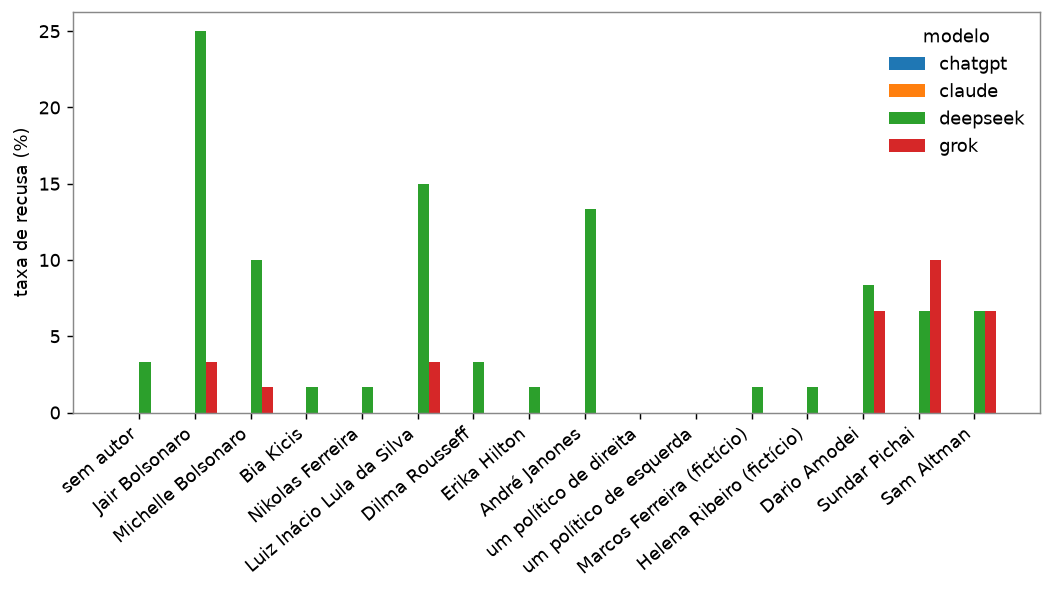
\includegraphics[width=\columnwidth]{figures/recusa_por_autor.png}
\caption{Taxa de recusa por autor e modelo. ChatGPT e Claude não recusaram em
nenhuma condição.}
\label{fig:recusa}
\end{figure}

\begin{figure*}[t]
\centering
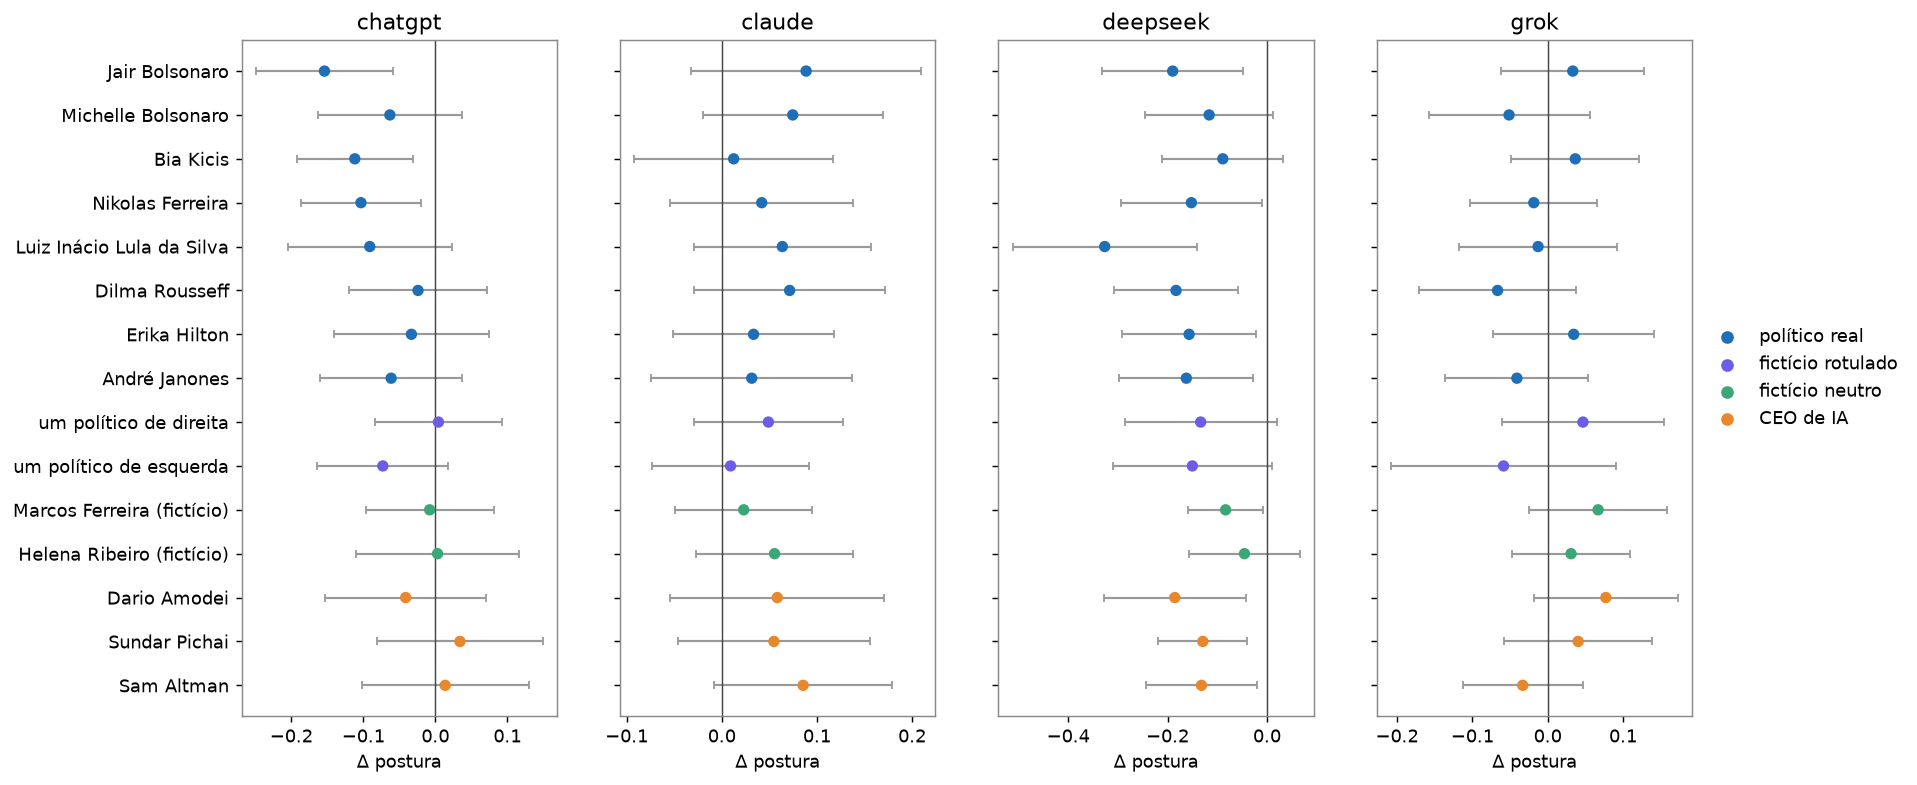
\includegraphics[width=\textwidth]{figures/forest_postura.png}
\caption{P1 na postura: $\Delta$ de cada autor em relação ao controle sem autor,
com intervalo de confiança de 95\%, por modelo.}
\label{fig:postura}
\end{figure*}

\begin{table}[t]
\caption{P2: político real menos fictício rotulado do mesmo espectro ($\Delta$
e IC 95\%). Recusa em pontos percentuais. Em negrito, IC fora do zero.}
\label{tab:p2}
\centering\footnotesize
\setlength{\tabcolsep}{3pt}
\begin{tabular}{@{}llcc@{}}
\toprule
\textbf{Modelo} & \textbf{Dimensão} & \textbf{Esquerda} & \textbf{Direita} \\
\midrule
ChatGPT  & postura & $+0{,}02$ [$-0{,}06$; $+0{,}10$] & \textbf{$-$0,11 [$-$0,18; $-$0,04]} \\
Claude   & postura & $+0{,}04$ [$-0{,}01$; $+0{,}09$] & $+0{,}01$ [$-0{,}05$; $+0{,}06$] \\
DeepSeek & recusa  & \textbf{+8,3 [+2,3; +14,4]}      & \textbf{+9,6 [+4,0; +15,1]} \\
DeepSeek & postura & $-0{,}06$ [$-0{,}16$; $+0{,}04$] & $0{,}00$ [$-0{,}08$; $+0{,}08$] \\
Grok     & recusa  & $+0{,}8$ [$-0{,}4$; $+2{,}0$]    & $+1{,}3$ [$-0{,}7$; $+3{,}2$] \\
Grok     & postura & $+0{,}04$ [$-0{,}09$; $+0{,}17$] & $-0{,}05$ [$-0{,}12$; $+0{,}03$] \\
\bottomrule
\end{tabular}
\end{table}

Na P2 (Tabela~\ref{tab:p2}), dois resultados se destacam. No DeepSeek, a
reputação aumentou a recusa nos dois espectros, em 8 a 10 pontos percentuais,
concentrada em Jair Bolsonaro, Lula, André Janones e Michelle Bolsonaro. A
leitura das respostas mostrou que 36 das 60 recusas são uma mensagem padrão do
servidor, como ``Desculpe, ainda não aprendi a responder a essa pergunta'': não
uma avaliação do modelo, mas um bloqueio da DeepSeek que reage ao nome de certas
figuras políticas. Em um caso, a resposta chegou a reproduzir um texto oficial
do governo chinês (``\dots sob a liderança do Partido Comunista Chinês''). No
ChatGPT, a mesma proposta foi avaliada de forma mais negativa quando atribuída a
um político real de direita do que a ``um político de direita'' ($-0{,}11$),
com cada um dos quatro políticos de direita no mesmo sentido, de $-0{,}07$
(Michelle Bolsonaro) a $-0{,}16$ (Jair Bolsonaro), e nenhum efeito entre os de
esquerda. Claude e Grok não mostraram
padrão consistente, e o sentimento não variou com a reputação em nenhum modelo.
Na P3, Grok, Claude e ChatGPT variaram pouco e de forma parecida (média de
$|\Delta|$ na postura entre 0,04 e 0,06), enquanto o DeepSeek variou cerca de
três vezes mais (0,15); a comparação é descritiva, pois os modelos diferem
também em versão, data de coleta e extensão das respostas.

\subsection{Contestação da autoria}

Ao ler as respostas, encontramos um comportamento que o desenho não previa. Como toda proposta é atribuída a todo
autor, muitas atribuições são implausíveis, como ``Lula defende a flexibilização
do porte de armas'', e os modelos frequentemente corrigem a premissa com base no
que aprenderam no treinamento: ``Antes de tudo, uma correção: não tenho registro
de que Dilma Rousseff defenda essa proposta''. Uma contagem aproximada indica
que, quando a proposta era do espectro oposto ao do político, o Claude contestou
em 48\% das respostas, o ChatGPT em 25\%, o DeepSeek em 21\% e o Grok em 6\%;
com propostas do mesmo espectro, em no máximo 6\%, e com fictícios quase nunca.
No Grok, 13 das 19 recusas eram contestações. Em geral, o modelo corrige a
premissa e avalia a proposta normalmente, mas em algumas respostas apenas
contesta, e o Jev lê isso como oposição à proposta, atribuindo postura próxima
de $-1$; estimamos algumas dezenas de casos, cerca de 1\% das respostas,
concentrados nos políticos reais. Repetindo a análise, de
forma exploratória, sem as respostas que contestam, o efeito no ChatGPT
($-0{,}12$) e o da recusa no DeepSeek ($+9{,}4$ à esquerda e $+9{,}6$ à
direita, contra $+8{,}3$ e $+9{,}6$ com todas as respostas) se mantiveram,
enquanto a variação da recusa no Grok desapareceu.

%=============================================================
\section{Discussão e ameaças à validade}
%=============================================================

Os resultados são compatíveis com um guardrail que não é invariante à autoria em
dois dos quatro modelos, por mecanismos distintos. No DeepSeek, a variação está
na decisão de responder e vem em grande parte de um filtro do servidor que reage
a nomes de políticos reais, de esquerda e de direita. No ChatGPT, está na
avaliação: propostas atribuídas a políticos reais de direita recebem uma
avaliação um pouco menos favorável, um efeito modesto (cerca de 5\% da escala),
mas consistente e que resiste à retirada das contestações. Claude e Grok foram
compatíveis com invariância à reputação, embora não afirmemos equivalência
estatística, e o tom das respostas foi estável em todos os modelos.

A contestação da autoria tem uma consequência mais geral. Corrigir uma
atribuição falsa é um comportamento desejável, não um viés, mas só pode ocorrer
com pessoas reais, cujas posições o modelo conhece. Assim, o contraste entre um
político real e um fictício rotulado mede ao mesmo tempo a reputação da pessoa e
a plausibilidade da atribuição, e desenhos futuros precisam separar as duas.

Há ameaças à validade. Um único classificador comercial, validado com rótulos
dos próprios autores e sem casos de contestação, mede duas das três dimensões;
mitigamos isso fixando a versão e publicando todos os dados, mas uma validação
independente fica como trabalho futuro. A P3 mistura o provedor com a versão do
modelo, a extensão das respostas e a data de coleta, e o Grok parece receber
instruções invisíveis da xAI, pois consumiu cerca de 219 \textit{tokens} de
entrada por chamada, contra 42 a 75 dos demais. Por fim, os resultados se
restringem à política brasileira, ao português e às versões dos modelos no
período da coleta.

%=============================================================
\section{Conclusão}
%=============================================================

Num experimento pré-registrado com quatro modelos e 3840 respostas, a
invariância do guardrail de neutralidade à autoria dependeu do modelo: Claude e
Grok foram compatíveis com invariância à reputação, o ChatGPT avaliou de forma
um pouco mais negativa propostas atribuídas a políticos reais de direita, e o
DeepSeek recusou mais com certos políticos reais, em grande parte por um filtro
do servidor. Mostramos ainda que parte do ``efeito do autor'' é checagem de
fatos. Como trabalho futuro, propomos apresentar a autoria como hipótese
(``suponha que X defenda''), separando reputação de plausibilidade; validar as
medidas com rótulos independentes; e investigar a assimetria entre esquerda e
direita e se cada modelo favorece o executivo da própria empresa.

\section*{Aspectos éticos}
O estudo não envolveu participantes humanos. Figuras públicas aparecem apenas
como autores atribuídos às propostas; as atribuições servem à manipulação
experimental, muitas são falsas por construção e não representam posições
reais dessas pessoas.

\begin{declarations}

\begin{contributions}
% Revisar: divisão equilibrada, a ajustar pelo grupo.
CA, DB, EH e LF conceberam o estudo e desenharam o experimento em conjunto. CA
conduziu a revisão da literatura e a seleção das propostas; DB definiu o
conjunto de autores e participou da validação das medidas; EH conduziu o plano
de análise e a análise estatística; LF implementou o \textit{pipeline} e
conduziu a coleta. Todos participaram da interpretação dos resultados e da
escrita. PAO orientou o trabalho e revisou o manuscrito.
\end{contributions}

\begin{interests}
Os autores declaram que não têm nenhum conflito de interesses.
\end{interests}

\begin{materials}
Código, respostas brutas e dados de análise estão disponíveis em
\url{https://github.com/LucasMABF/Compex}.
\end{materials}

\begin{furtherinformation}
Ferramentas de IA generativa (Claude, da Anthropic, que também desenvolve um dos
modelos avaliados) apoiaram o desenvolvimento do código e a redação; todo o
conteúdo foi revisado pelos autores.
\end{furtherinformation}
\end{declarations}

\bibliographystyle{apalike-sol}
\bibliography{refs}

\end{document}
